% !TEX TS-program = pdflatex
% !TEX encoding = UTF-8 Unicode

% This is a simple template for a LaTeX document using the "article" class.
% See "book", "report", "letter" for other types of document.

\documentclass[11pt]{article} % use larger type; default would be 10pt

\usepackage[utf8]{inputenc} % set input encoding (not needed with XeLaTeX)

%%% Examples of Article customizations
% These packages are optional, depending whether you want the features they provide.
% See the LaTeX Companion or other references for full information.

%%% PAGE DIMENSIONS
\usepackage{geometry} % to change the page dimensions
\geometry{a4paper} % or letterpaper (US) or a5paper or....
% \geometry{margin=2in} % for example, change the margins to 2 inches all round
% \geometry{landscape} % set up the page for landscape
%   read geometry.pdf for detailed page layout information

\usepackage{graphicx} % support the \includegraphics command and options

% \usepackage[parfill]{parskip} % Activate to begin paragraphs with an empty line rather than an indent

%%% PACKAGES
\usepackage{booktabs} % for much better looking tables
\usepackage{array} % for better arrays (eg matrices) in maths
\usepackage{paralist} % very flexible & customisable lists (eg. enumerate/itemize, etc.)
\usepackage{verbatim} % adds environment for commenting out blocks of text & for better verbatim
\usepackage{subfig} % make it possible to include more than one captioned figure/table in a single float
% These packages are all incorporated in the memoir class to one degree or another...

%%% HEADERS & FOOTERS
\usepackage{fancyhdr} % This should be set AFTER setting up the page geometry
\pagestyle{fancy} % options: empty , plain , fancy
\renewcommand{\headrulewidth}{0pt} % customise the layout...
\lhead{}\chead{}\rhead{}
\lfoot{}\cfoot{\thepage}\rfoot{}

%%% SECTION TITLE APPEARANCE
\usepackage{sectsty}
\allsectionsfont{\sffamily\mdseries\upshape} % (See the fntguide.pdf for font help)
% (This matches ConTeXt defaults)

%%% ToC (table of contents) APPEARANCE
\usepackage[nottoc,notlof,notlot]{tocbibind} % Put the bibliography in the ToC
\usepackage[titles,subfigure]{tocloft} % Alter the style of the Table of Contents
\renewcommand{\cftsecfont}{\rmfamily\mdseries\upshape}
\renewcommand{\cftsecpagefont}{\rmfamily\mdseries\upshape} % No bold!

%%% END Article customization
\usepackage{graphicx}
\graphicspath{{images/}}
\usepackage[english]{babel}
\usepackage{multirow}

%%% The "real" document content comes below...

\title{4x4x4 LED Cube\\
\large Final Project Proposal}
\author{Grant Gunnison}
%\date{} % Activate to display a given date or no date (if empty),
         % otherwise the current date is printed 

\begin{document}
\maketitle

\section{Background}

A couple of years ago I thought it would be a really cool idea to build an LED cube, but at the time had absolutely no idea how to build it. After taking 6.131 and now 6.115, my lab skills have gotten much better with regards to electronics and I now feel confident that I could actually build it so I figured it would be fun make this my final project. I bought the stuff for the cube at the beginning of this semester and have very casually been working on it ~ a couple hours a week at most. I have made some progress, but likely have a 100+ more hours to put into it before it is functional. The cube is a lattice of connected common anode LED's that form an 8x8x8 led cube structure. Each horizontal level is commonly connected and each vertical column is connected. By multiplexing the horizontal levels at a frequency $>$30 Hz the cube looks as if all of the levels are being controlled at the same time, given the illusion of the cube having individually addressable LED's, while LED's can only be controlled one level at a time in reality.

\section{Hardware Description}

The amount of hardware that it takes to build an 8x8x8 cube is actually fairly enormous. The list includes:

\begin{enumerate}
\item 512 5mm LEDS
\item 200 NPN transistors
\item 401 1K resistors
\item 328 100 ohm resistors
\item 8 PNP mosfets
\item 25 shift registers
\item 30 .1 uF capacitors
\item 200+ ft of 22 AWG wire
\end{enumerate}


For this reason I will build the 8x8x8 lattice structure, but only control a 4x4x4 piece of the larger cube. The amount of wiring is prohibitive in the amount of time that I have.\\

Figure 1 shows a schematic of the control hardware layout. Due to the size of the project I chose not to build out the entire 8x8x8 cube's control hardware. The anode (horizontal slices) control circuit controls one level of the cube (out of the 8) at a time. Each shift register will control a PFET that will source the necessary amount of current to the level (Figure 2). Each cathode will control a single LED which have $BL_IN$ labels in the schematic. Each Cathode will be connected to a control circuit that is shown in Figure 3. There are three colors shown, but this project will only connect the red color. To turn on any LED both its horizontal level must be turned on as well as the corresponding cathode.

\begin{figure}[h]
\caption{Shift Register}
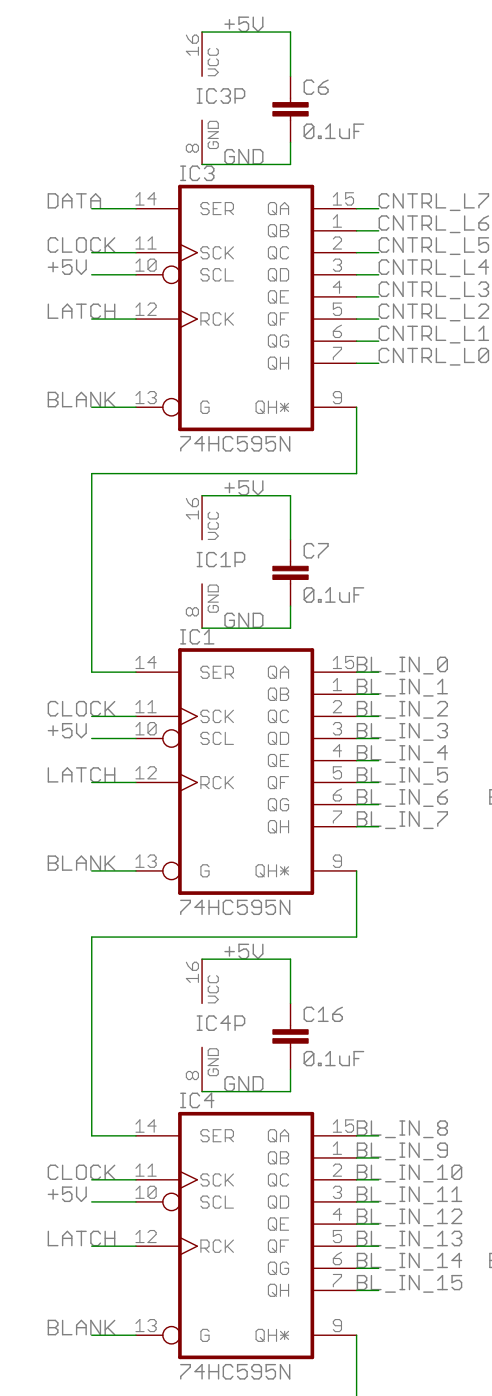
\includegraphics[scale=.75]{Schematic}
\centering
\end{figure}

\begin{figure}[!htb]
\caption{Anode control Circuit}
\includegraphics[scale=.75]{anode}
\centering
\end{figure}

\begin{figure}[!htb]
\caption{Cathode control Circuit}
\centering
\includegraphics[scale=.5]{blue}
\includegraphics[scale=.5]{red}
\includegraphics[scale=.5]{green}
\end{figure}

The cube will be controlled using the 8051 or the PSOC. At this point it is not clear how difficult it will be to write the code in .ASM and am giving myself the flexibility to write it in C if I choose to do that. The processor that is not controlling the cube will be used to control a LCD display the name of the graphic on the cube, or the number of LED's that are currently on at any given time. 


\section{Software Description}

The software control is overall conceptually fairly simple, but the semantics involved with getting interesting and cool images to appear on the cube will be pretty challenging. The way the cube is controlled is level by level. On each level the shift registers are filled with 1's and 0's which are connected to corresponding LED's. 1's turn on an LED and 0's turn it off. All 16 bits must be pushed into the registers and then each one is latched to output which will turn on the led's. After it is latched, new data is pushed and then next level is activated.The levels are cycled through to appear as if all of the them are on simultaneously.
\newline
\newline
With the basic concept down, the real challenge will be to display cool graphics. The overall goal of this cube is to be able to display some rotating images of some sort and will require either extensive data bases, or large hardcoded loops to display all of the images.

\section{Project Scope}
I believe the 8x8x8 cube is by leaps and bounds much more difficult from both a hardware and software perspective than any of the labs we have done thus far and is probably on the order of 5x the complexity of the other labs. Therefore I scaled the project back significantly by only controlling one color and only one 4x4x4 quadrant of the entire cube. This siginficantly reduces the size of the software package as well as the amount of control hardware that needs to be built. 
\newline
\newline
All this being considered I believe that an "A" level project will be to have the 4x4x4 cube fully functional with at least one rotating or periodic image and the LCD display showing the name of the image being displayed. A "B" level project will have the cube function, but will only display static images and have the LCD display showing the name of the display. A "C" level project will be to have the cube finished, but only have marginal images or only a few LEDs be lit up at a time, nothing that provides a wow factor.
\section{Special Components}
For the time being, I have already purchased everything that I believe I need.

\section{Timetable}
\begin{center}
	\begin{tabular}{ | c | c | }
	\hline
	Date & Objective \\ \hline
	April 11 & Finish design \\ \hline
	April 18 & Finish building the cube and all control hardware \\ \hline
	April 25 & Build and get simple software program working \\ \hline
	May 2  & Continue to build software and integrate other peripherals get simple image working\\ \hline
	May 9 & Get more complex images working and debug \\ \hline
	\end{tabular}
\end{center}




\end{document}
